% !TeX spellcheck = da_DK
\section{Samlet systemtest}
Efter de enkelte blokke blev testet og godkendt hver for sig, skal det samlede system testes. Formålet med den samlede systemtest er at kontrollere, hvorvidt systemet overholder de overordnede funktionelle krav jævnfør afsnit \ref{FunkKrav} på side \pageref{FunkKrav}. Der anvendes samme fremgangsmåde for test af det samlede system, som af de øvrige blokke; Først simuleres systemet i LTspice, hvorefter det implementeres og testes. Det samlede system vil blive testet på to forskellige måder - først en test efter samme principper som i testen af accelerometeret og efterfølgende en test, hvor accelerometeret er placeret på en person jævnfør afsnit \ref{formaal_anvendelse} på side \pageref{formaal_anvendelse}.

\subsection{Simulering}
I simuleringen af det samlede system kontrolleres det, som i de øvrige simuleringer, om systemet fungerer med ideelle komponenter. Denne kontrol udføres ved at indsende en sinus som inputspænding igennem systemet, som teoretisk skal aktivere hhv. de enkelte dioder og vibratorerne. Designet af det samlede system ses på \figref{fig:samlet_system}:
\begin{figure}[H]
	\centering
	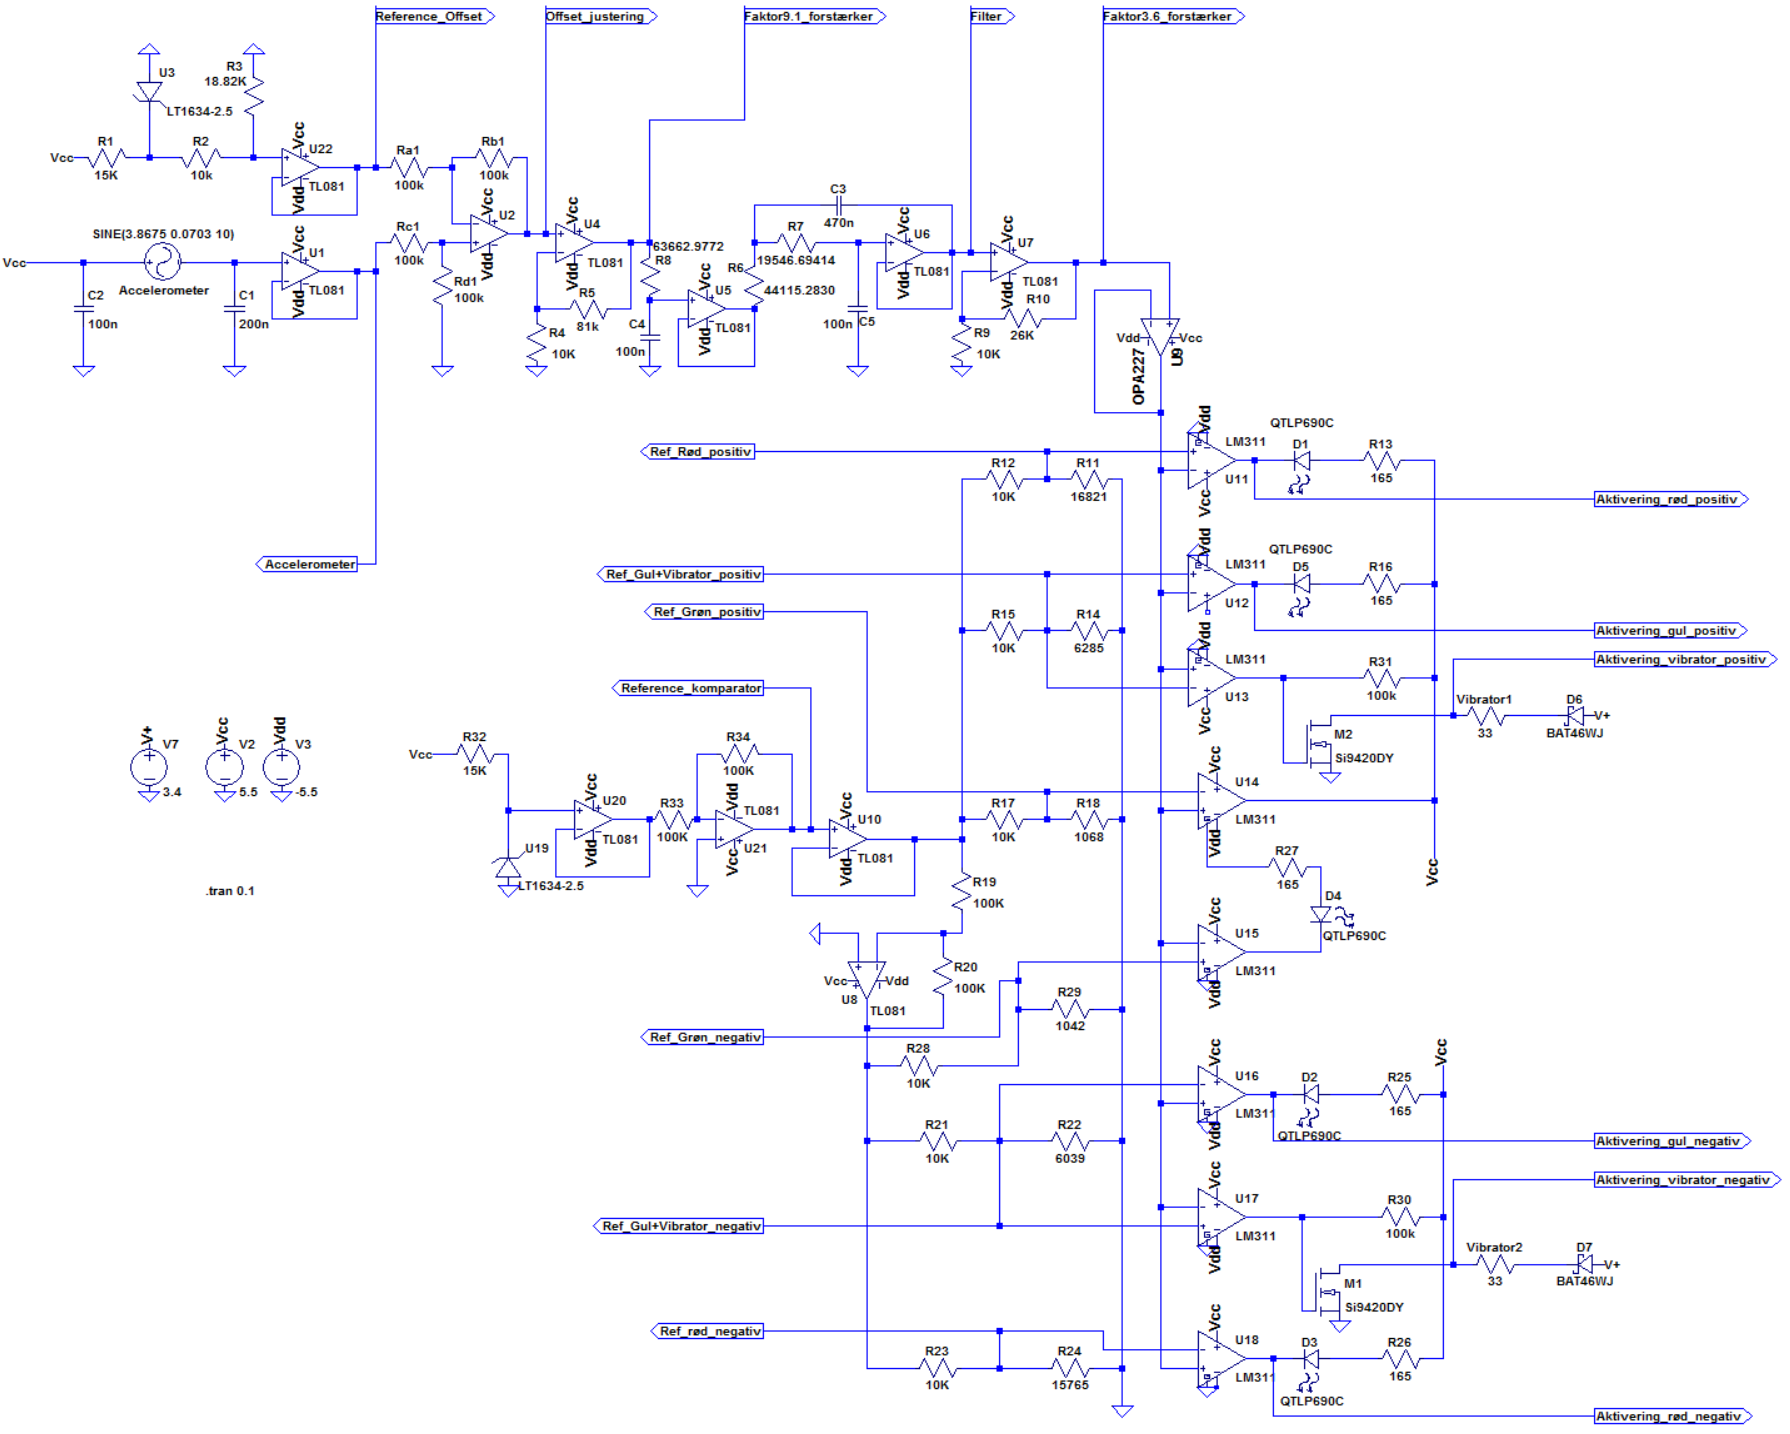
\includegraphics[scale=.3]{figures/cProblemloesning/Samlet_system.PNG}
	\caption{På figuren ses designet af det samlede system med labels, der indikerer målepunkterne for de følgende simuleringer. Derved kan blokkenes påvirkning af signalet følges undervejs i systemet.}
	\label{fig:samlet_system}
\end{figure}
\noindent Sinussignalets amplitude udregnes til at være:
\begin{eqnarray}
0.0037 \cdot (\dfrac{(25-13)}{2} + 13) = 0.0703V
\end{eqnarray}
$0.0037$V er den maksimale spænding fra accelerometret ved $1^{\circ}$ hældning. Dette ganges med $19$, hvilket er midterpunktet for aktivering af en rød diode ($13^{\circ}$) og mætning af den sidste forstærker ($25^{\circ}$). Der fås en amplitude på $0.0703$V. Det kan derved måles, om systemet teoretisk opfylder de overordnede funktionelle krav jævnfør afsnit \ref{FunkKrav} på side \pageref{FunkKrav}.\\
I simuleringen af dette system måles inputtet fra accelerometret og outputtet for hver af feedback komponenterne. Dette ses på \figref{fig:samlet_system_simulering}:
\begin{figure}[H]
	\centering
	\includegraphics[scale=.3]{figures/cProblemloesning/Samlet_system_simulering.PNG}
	\caption{...}
	\label{fig:samlet_system_simulering}
\end{figure}

\subsection{Implementering}

\subsection{Test 1}
I den første test af det samlede system tages udgangspunkt i principperne fra testen af accelerometeret beskrevet i afsnit \ref{Acc_afsnit} på side \pageref{Acc_afsnit}. Det måles således, hvorvidt systemet opfylder de overordnede funktionelle krav jævnfør afsnit \ref{FunkKrav} på side \pageref{FunkKrav}, ved at placere accelerometeret i de definerede hældningsgrader, og herudfra vurdere om den korrekte feedback udløses.  

\subsection{Test 2}
I den anden test af det samlede system placeres accelerometeret i stedet på en forsøgsperson, der skal afprøve træningsforløbet med systemet. Formålet med denne test er igen at kontrollere om den korrekte feedback udløses, samt at vurdere, hvorvidt de definerede hældningsgrader er passende under træning med systemet. 
 